\documentclass{beamer}
%\usepackage{beamerthemelined}
\usepackage{amsfonts,amssymb,amsmath}
\usepackage{graphicx}
\usepackage{animate}

\usetheme{Boadilla}
\usecolortheme{whale}
\beamertemplatenavigationsymbolsempty
\setbeamertemplate{itemize items}[triangle]
\setbeamertemplate{footline}[frame number]

\newcounter{conclusion}
\newcommand\conclude{\addtocounter{conclusion}{1}Conclusion \#\arabic{conclusion}}

\newcommand\myciteetal[3]{{\small #1 \emph{et al}, \textit{#2} (#3)}}
\newcommand\mycite[3]{{\small #1, \textit{#2} (#3)}}
\newcommand\rr{\mathbf{r}}

\title{A Tale of Two E's}
\subtitle{Energy and Entropy in liquid interfaces}
\author{David Roundy}
\date{2013}

\AtBeginSection[]
{
  \begin{frame}
    \frametitle{Outline}
    \tableofcontents[currentsection]
  \end{frame}
}

\begin{document}

{
%\usebackgroundtemplate{\includegraphics[height=\paperheight]{photos/montage}}%
\begin{frame}
  \titlepage
  %\vfill

  %\hfill \includegraphics[width=4cm]{figs/nsf-due-0837829}
\end{frame}
}

\begin{frame}
  \frametitle{How are energy and entropy involved?}
  \vspace{-1em}
  \[F = U - TS\]
  \begin{center}
    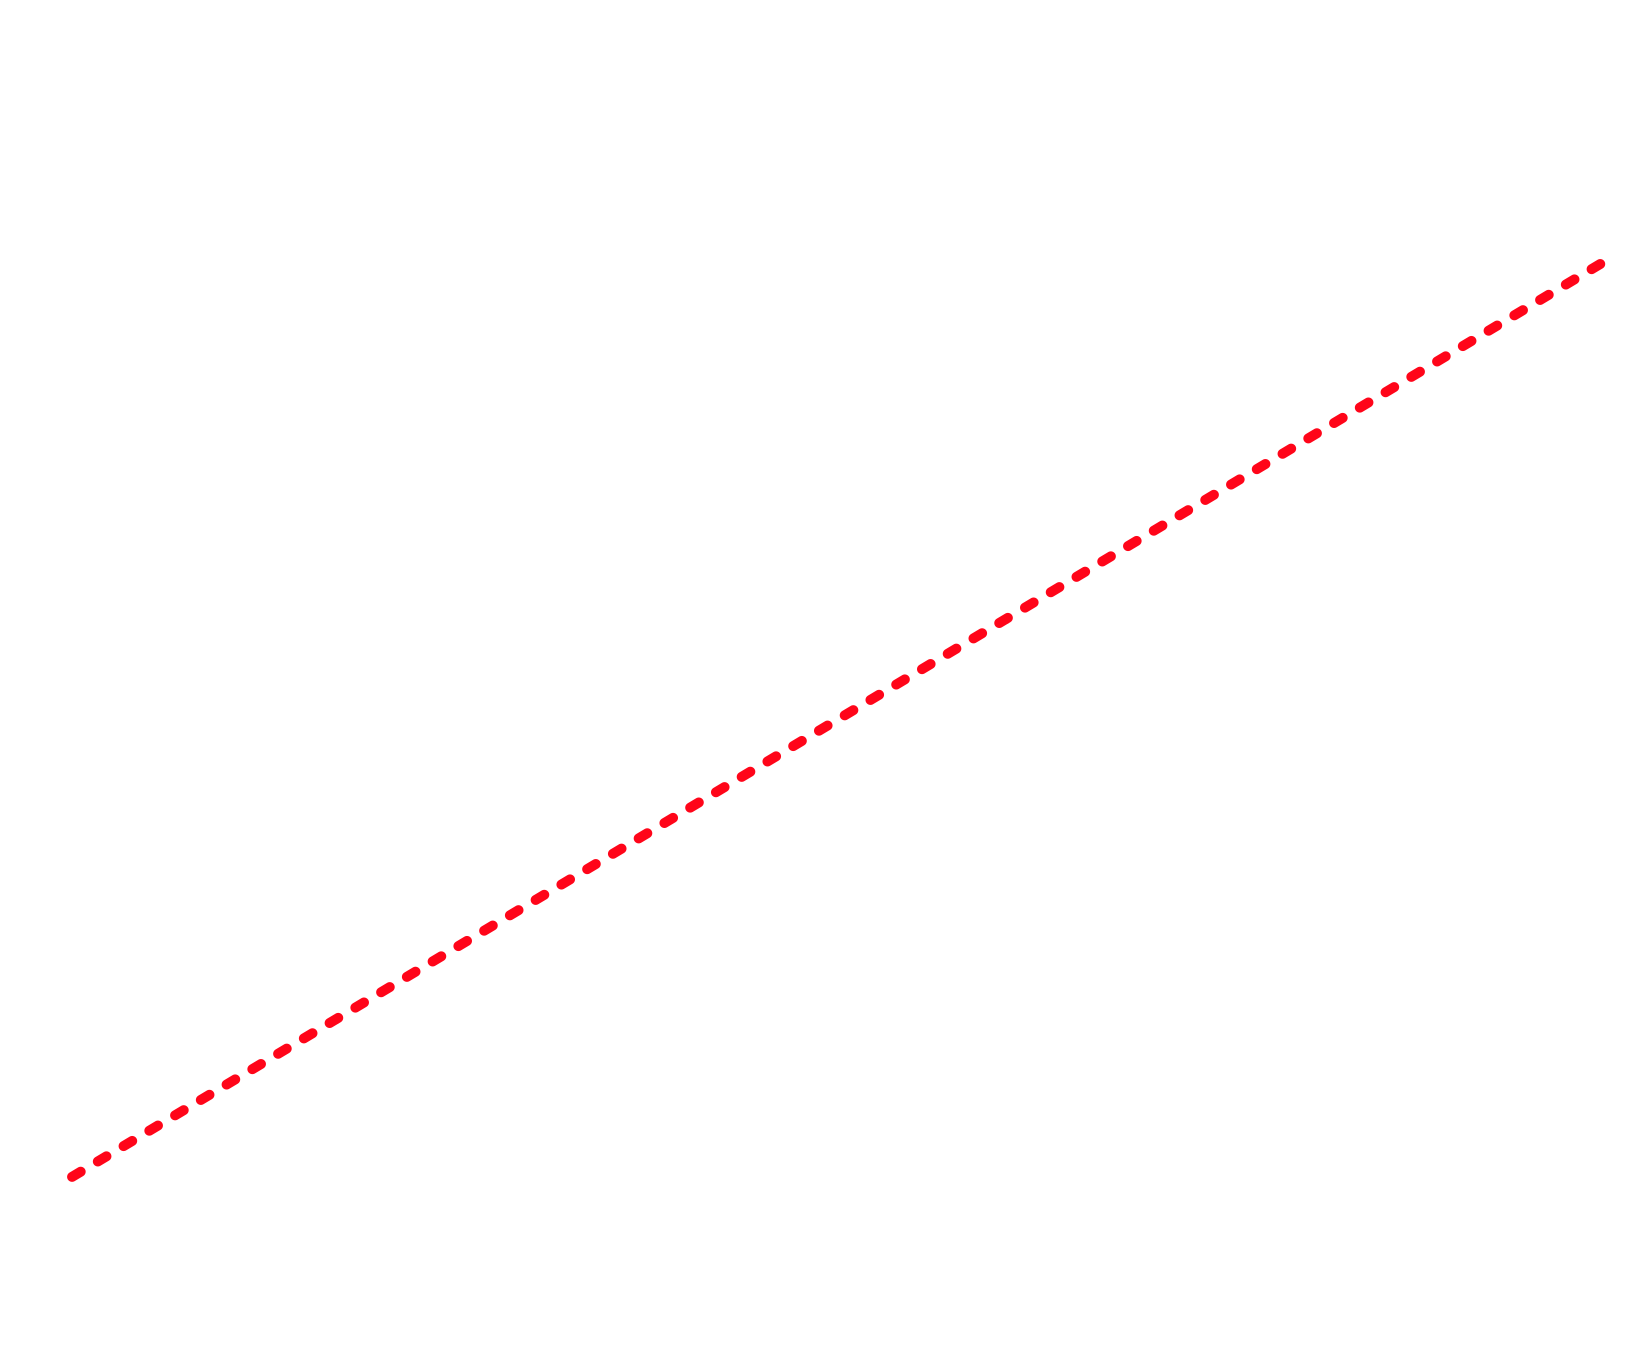
\includegraphics[height=6cm]{figs/hydration-plot-nice}
  \end{center}
  ``The energy and entropy of hydration of organic compounds''
  \\ \hfill \mycite{Butler}{Transactions of the Faraday Society}{1937}
\end{frame}

%\section*{Outline}
\begin{frame}
  \frametitle{Outline}
  \tableofcontents
\end{frame}

\section{Theory of Liquids}
\subsection*{What is a liquid?}
\begin{frame}
  \frametitle{What is a liquid?}
  \framesubtitle{Elementary school definition}
  \begin{center}
    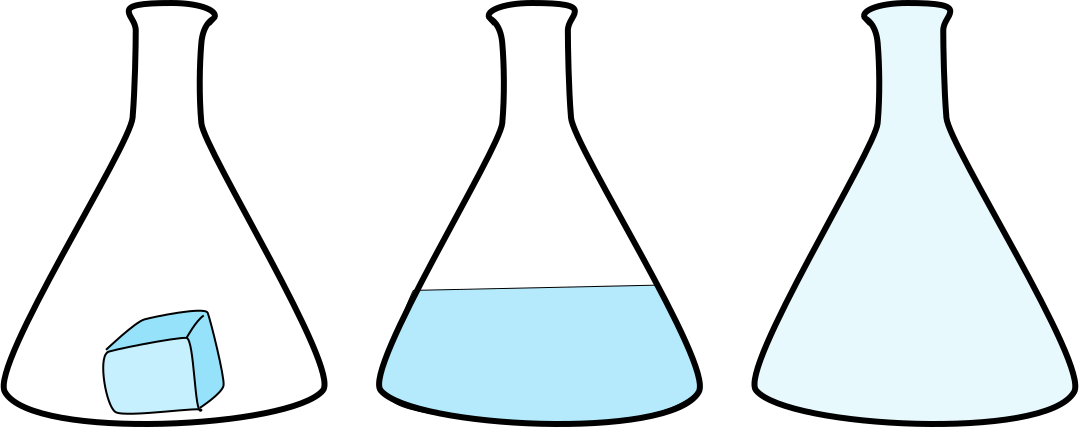
\includegraphics[width=7cm]{figs/solid-liquid-gas}
  \end{center}
  \begin{description}
  \item[Solid] Does not take the shape of its container
  \item[Gas] Takes the shape of its container and fills it
  \item[Liquid] Takes the shape of a container, but doesn't fill it
  \end{description}
\end{frame}

\begin{frame}
  \frametitle{What is a liquid?}
  %\framesubtitle{Phase diagram}
  \begin{center}
    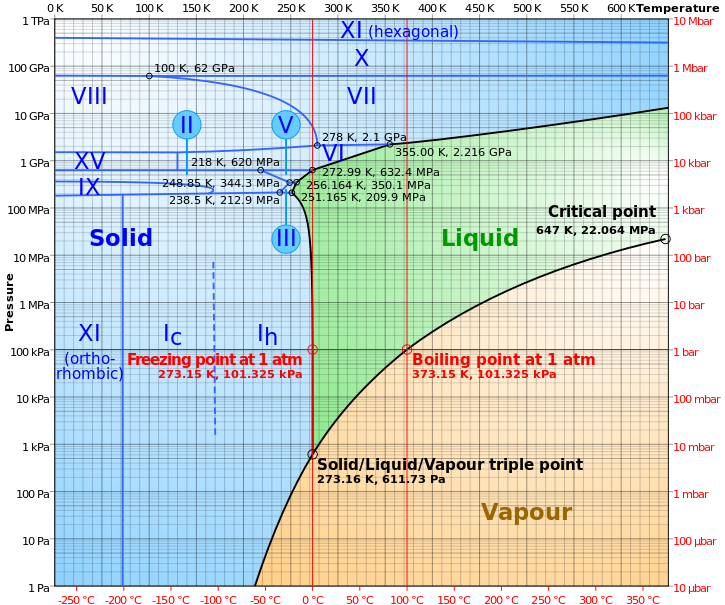
\includegraphics[width=8.8cm]{figs/water-phase-diagram}
  \end{center}
  \vspace{-1em}
  \hfill \tiny figure from Wikipedia
\end{frame}

\begin{frame}
  \frametitle{What is a liquid?}
  \framesubtitle{Energy versus entropy}
  \begin{center}
    \includegraphics<1>[width=7cm]{figs/energy-solid}
    \includegraphics<2>[width=7cm]{figs/energy-solid-gas}
    \includegraphics<3->[width=7cm]{figs/energy-solid-gas-liquid}
  \end{center}
  \begin{description}
  \item[Solid] Energy dominates, entropy is a small perturbation
  \item<2->[Gas] Entropy dominates, energy is a small perturbation
  \item<3->[Liquid] Energy and entropy are balanced
  \end{description}
  \begin{block}{Perturbation theory}<4->
    \begin{itemize}
    \item<5-> An ``easy'' problem we know how to solve
    \item<6-> A ``hard'' correction that is small
    \item<7-> We construct a power series to solve combined problem
    \end{itemize}
  \end{block}
  %% \begin{enumerate}
  %% \item Solid and gas perturbation expansion
  %% \item No easy perturbation for liquid
  %% \item Ice floats
  %% \item Critical point
  %% \item Below the triple point
  %% \end{enumerate}
\end{frame}

%% \section[SAFT]{Understanding water using Statistical Associating
%%   Fluid Theory}

%% \subsection*{Simple liquids}
%% \begin{frame}
%%   \frametitle{Dense fluids}
%%   In order to use a perturbative approach, we need a ``solved''
%%   problem that is similar to a liquid.

%%   \begin{block}{Correlation function}<2->
%%     \vspace{-3em}
%%     \hfill \includegraphics[width=5cm, angle=270]{figs/correlation}\\
%%     %\vspace{-1em}
%%     \hfill\mycite{Soper}{J. Chem. Phys.}{2000}\\
%%     The correlation function $g(r)$ tells us how likely we are to find
%%     an atom at a given distance from any other atom.
%%   \end{block}
%% \end{frame}

\begin{frame}
  \frametitle{Dense fluids}
  In order to use a perturbative approach, we need a ``solved''
  problem that is similar to a liquid.
  \begin{block}{Hard-sphere fluid}<2->
    \begin{itemize}
    \item Captures the repulsive portion of the structure
    \item Still no energy!
    \item Not actually a liquid
    \end{itemize}
    \begin{center}
      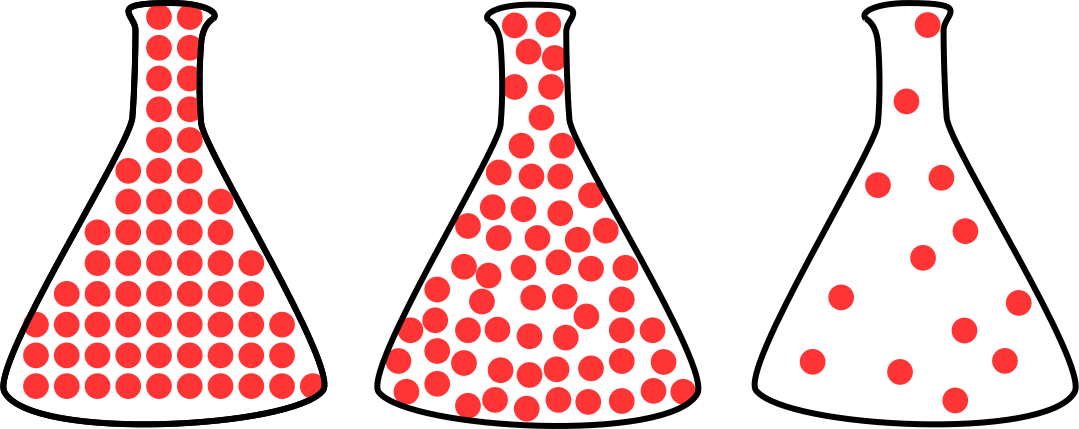
\includegraphics[width=8cm]{figs/hard-spheres}
    \end{center}
  \end{block}
\end{frame}

\begin{frame}
  \frametitle{Simple liquids}
  \begin{itemize}
  \item Perturbative attraction added to hard spheres
  \item ``High T expansion''
    \[
    F_\text{disp} = N\left(a_1(n) + a_2(n)\beta + \mathcal{O}(\beta^2)\right),
    \quad \quad \beta \equiv \frac{1}{k_BT}
    \]

    \vspace{1em} The temperature-independent $a_1$ term corresponds to
    a mean-field approximation, and incorporates correlations present
    in the hard-sphere fluid.
    \vspace{1em}

    The $a_2$ term incorporates---to first order---correlations due to
    the attraction itself.
  \end{itemize}
\end{frame}

%\subsection{Hydrogen bonding (Association)}
\begin{frame}
  \frametitle{Hydrogen bonds (Association)}
  \vspace{-2em}
  \hfill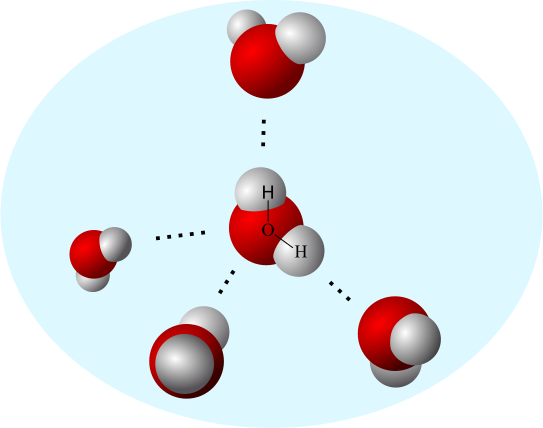
\includegraphics[width=7cm]{figs/hydrogen-bonds}\hspace{-3em}
  \vspace{-2em}
  \begin{itemize}
  \item Highly directional bonds
  \item Not a ``small'' interaction (around $4k_BT$)
  \item Small volume of interaction
  \item Wertheim's Thermodynamic Perturbation Theory\\ \hfill
    \mycite{Wertheim}{J. Stat. Phys.}{1984,1986}
  \end{itemize}
\end{frame}

\begin{frame}
  \frametitle{Putting it all together}
  All these terms combined describe SAFT, a well-established theory
  for \emph{homogeneous} liquids such as water.
  \begin{center}
    \vspace{-1em}
    \includegraphics[height=6cm]{../../papers/water-saft/figs/pressure-with-isotherms-truncated}
  \end{center}
  \hfill Clark \emph{et al}, \emph{Mol. Phys.}
  (2006)
\end{frame}

\begin{frame}
  \frametitle{Interfaces:  Classical Density Functional Theory}
  In order to describe liquid \emph{interfaces} we need a theory that
  can handle \emph{inhomogeneous} configurations.
  \begin{block}{Classical Density Functional Theory (cDFT)}
    \[\Omega = \min_{n(\rr)} \left\{ F[n(\rr), T] + \int (V(\rr)-\mu) n(\rr)d\rr \right\}
    \]
    \begin{itemize}
    \item $\Omega$ is grand potential
    \item $n(\rr)$ is number density of atoms or molecules
    \item $V(\rr)$ is an arbitrary external potential energy
    \item $\mu$ is the chemical potential
    \item $F[n(\rr),T]$ is a functional that depends only on the
      liquid in question
    \end{itemize}
  \end{block}
\end{frame}

\begin{frame}
  \frametitle{Testing the theory:  Monte Carlo simulation}
  \vspace{-0.8em}
  \begin{center}
    \animategraphics[height=20em]{.6}{anim/mc-slow-}{000}{30}\\
    \vspace{-2.0em}
    hard circles between two walls
  \end{center}
\end{frame}

\begin{frame}
  \frametitle{Testing the theory:  Monte Carlo simulation for $n(\rr)$}
  \vspace{-0.8em}
  \begin{center}
    \animategraphics[height=20em,autoplay]{.6}{anim/mc-density-}{000}{30}\\
    \vspace{-2.0em}
    hard circles between two walls
  \end{center}
\end{frame}



\section{Association:  making contact}
\subsection*{}

\begin{frame}
  \frametitle{How often do hard spheres touch?}

  A key input to Wertheim's TPT is the contact value of the
  correlation function of the hard-sphere fluid.
  \begin{itemize}
  \item<2-> Well known for a homogeneous fluid
  \item<2-> Two approximate functions for inhomogeneous systems
    \\ \hfill \mycite{Yu and Wu}{J. Chem. Phys.}{2002}\tiny ;
    \mycite{Gross}{Surface Science}{2002}
  \item<2-> Little justification, and no testing!
  \end{itemize}
  \begin{block}{}<3->
  \begin{center}
    
\includegraphics[height=3cm]{figs/HaglundChris}
    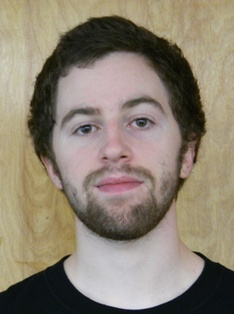
\includegraphics[height=3cm]{figs/KreitzbergPatrick}
    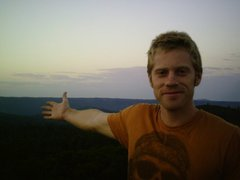
\includegraphics[height=3cm]{figs/SchulteJeff}
  \end{center}
  \end{block}
\end{frame}

\begin{frame}
  \frametitle{Finding the distribution function at contact $g_\sigma$}
  \vspace{-0.8em}
  \begin{center}
    \animategraphics[height=20em,autoplay]{.6}{anim/mc-gsigma-}{000}{30}\\
    \vspace{-2.0em}
    hard circles between two walls
  \end{center}
\end{frame}

\begin{frame}
  \frametitle{Monte Carlo:  spheres at a hard wall}
  \begin{columns}
    \begin{column}{0.5\columnwidth}
      \begin{center}
        low density\\
        \includegraphics[width=1.1\columnwidth]{figs/walls-mc-10}
      \end{center}
    \end{column}
    \begin{column}{0.5\columnwidth}
      \begin{center}
        high density\\
        \includegraphics[width=1.1\columnwidth]{figs/walls-mc-40}
      \end{center}
    \end{column}
  \end{columns}
\end{frame}

\begin{frame}
  \frametitle{Our theoretical approach}
  \begin{block}{Contact value theorem}
    Pressure on any hard surface is determined by the density of
    molecules in contact with it:
    \vspace{-1em}
    \[ p = n_{c}k_BT \]
    \vspace{-2em}
    \begin{itemize}
    \item We find pressure on spheres from a free energy derivative
      \vspace{-0.5em}
      \[p = \frac{1}{n(\rr)}\frac{1}{4\pi(2R)^2}\frac{\delta F_{HS}}{\delta R(\mathbf{r})}\]
    \item From the pressure, we know the density at contact
    \item From the density at contact, we find the correlation
      function
      \vspace{-0.5em}
      \[g_\sigma^A(\rr)
      = \frac{1}{n(\rr) n_A(\rr)}\frac{1}{ k_BT 4\pi (2R)^2} \frac{\delta
        F_{HS}}{\delta R(\mathbf{r})}\]
      \[
      n_A(\rr) = \int n(\rr')
      \frac{\delta(2R -|\rr-\rr'|)}{4\pi(2R)^2} d\rr' \label{eq:nA}
      \]
    \end{itemize}
  \end{block}
\end{frame}

\begin{frame}
  \frametitle{Results}
  \begin{center}
    Hard spheres at a hard wall, 10\% packing fraction\\
    \includegraphics[height=7cm]{figs/walls-10}
  \end{center}
\end{frame}

\begin{frame}
  \frametitle{Results}
  \begin{center}
    Hard spheres at a hard wall, 40\% packing fraction\\
    \includegraphics[height=7cm]{figs/walls-40}
  \end{center}
\end{frame}

\begin{frame}
  \frametitle{\conclude}
  \begin{center}
    \includegraphics[height=4cm]{figs/walls-10}
    \includegraphics[height=4cm]{figs/walls-40}
  \end{center}
  \begin{itemize}
  \item Derived and tested an accurate functional for the correlation
    function at contact for hard spheres
  \item Reasonably efficient: scales like the hard sphere free energy
  \end{itemize}
\end{frame}



\section{Dispersion: pair distribution function}

\subsection{}

\begin{frame}
  \frametitle{Finding the pair distribution function $g^{(2)}(\rr_1,\rr_2)$}
  \begin{figure}[h]
    \centering
    \animategraphics[width=100mm,autoplay,final]{2.0}{anim/mc-pair-}{000}{30}
  \end{figure}
\end{frame}



\section{Putting it all together: water}

\subsection{}

\begin{frame}
  \frametitle{Putting it all together}
  \begin{center}
    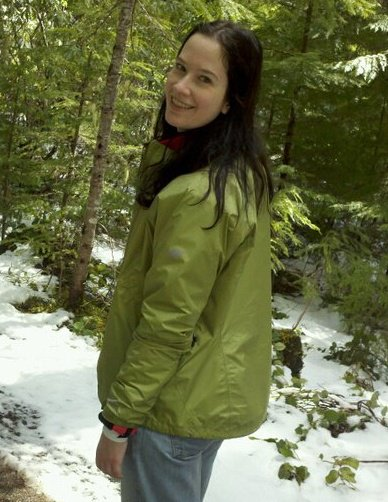
\includegraphics[height=3cm]{figs/HughesJessica}
    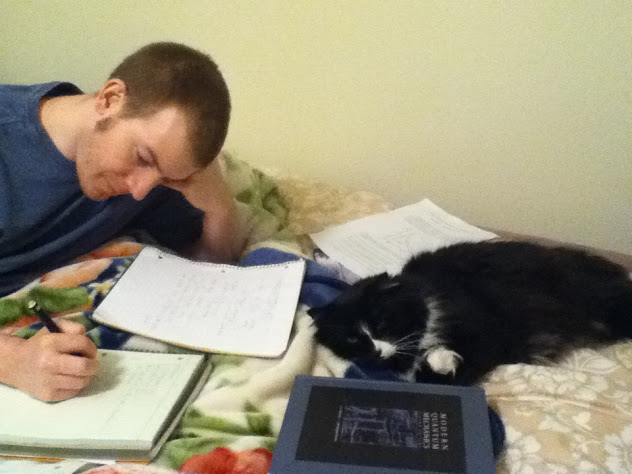
\includegraphics[height=3cm]{figs/KrebsEric}
  \end{center}
  \begin{block}{Statistical Associating Fluid Theory}
    \[
    F = F_{\textit{ideal gas}} + F_{\textit{hard spheres}} + F_{\textit{dispersion}} + F_{\textit{association}}
    \]
    We combine these terms to produce a classical density functional
    describing water.
  \end{block}
\end{frame}

\begin{frame}
  \frametitle{Homogeneous limit}
  \begin{center}
    \vspace{-1em}
    \includegraphics[height=6cm]{../../papers/water-saft/figs/pressure-with-isotherms-truncated}
   \end{center}
  Five SAFT empirical parameters taken from\\\hfill Clark \emph{et al.}, \emph{Mol. Phys.}
  (2006)
\end{frame}

\begin{frame}
  \frametitle{Homogeneous limit}
  \begin{center}
    \vspace{-1em}
    \includegraphics[height=7cm]{../../papers/water-saft/figs/surface-tension}
  \end{center}
  \vspace{-1.5em}
  One additional empirical parameter (in dispersion) used to fit
  surface tension.
\end{frame}

%% \begin{frame}
%%   \frametitle{Two hard rods}
%%   \begin{center}
%%     \vspace{-1em}
%%     \includegraphics[height=8cm]{figs/density-rods-in-water}
%%   \end{center}
%%   \vspace{-1.5em}
%% \end{frame}

\begin{frame}
  \frametitle{Hydration of a hard sphere}
  \begin{center}
    \vspace{-1em}
    %\includegraphics[height=7cm]{figs/sphere-energy-vs-diameter}
  \end{center}
  \vspace{-1.5em}
\end{frame}

\begin{frame}
  \frametitle{Conclusion \#2}
  \vspace{2em}
  \begin{block}{Hard sphere contact}
    \vspace{-6em}
    \hfill
    \includegraphics[height=2cm]{figs/walls-10}
    \includegraphics[height=2cm]{figs/walls-40}
    \begin{itemize}
    \item Found and tested an accurate functional for the correlation
      function at contact for hard spheres
    \item Reasonably efficient: scales like the hard sphere free
      energy
    \end{itemize}
  \end{block}
  \begin{block}{Water}
    \begin{itemize}
    \item Developed and tested a SAFT-based functional for water
    \end{itemize}
  \end{block}
  \begin{block}{Future work}
    \begin{columns}
      \begin{column}{0.7\columnwidth}
        \begin{itemize}
        \item Test dispersion versus MC
        \item Renormalization group for critical point
        \item Hard polyhedra for directional correlation
        \end{itemize}
      \end{column}
      \begin{column}{0.5\columnwidth}
        \begin{itemize}
        \item Dielectric interactions
        \item Softening the spheres
        \item Coupling with solute
        \end{itemize}
      \end{column}
    \end{columns}
  \end{block}
\end{frame}



\end{document}
